%%%%%%%%%%%%%%%%%%%%%%%%%%%%%%%%%%%%%%%%%%%%%%%%%%%%%%%%%%%%%%%%%%%%%%%%%%%%%%%%%%%
%% This project aims to create the template for presentation.                   %%
%% author: Luigi Durso                                                          %%
%% contacts:                                                                    %%
%%    e-mail: luigi.durso@si2001.it                                             %%
%%    linktree: https://linktr.ee/maumneto                                      %%
%%%%%%%%%%%%%%%%%%%%%%%%%%%%%%%%%%%%%%%%%%%%%%%%%%%%%%%%%%%%%%%%%%%%%%%%%%%%%%%%%%%
\documentclass{../libs/presentation_format}
% Inserting the preamble file with the packages
%%%%%%%%%%%%%%%%%%%%%%%%%%%%%%%%%%%%%%%%%%%%%%%%%%%%%%%%%%%%%%%%%%%%%
%% This file contains the packages that can be used in the beamer. %%
%%%%%%%%%%%%%%%%%%%%%%%%%%%%%%%%%%%%%%%%%%%%%%%%%%%%%%%%%%%%%%%%%%%%%
% Package to fonts family
\usepackage[T1]{fontenc}
% Package to accentuation
\usepackage[utf8]{inputenc}
% Package to Italian language
\usepackage[italian]{babel}
% Package to Figures
\usepackage{graphicx}
\usepackage{caption}
\usepackage{subcaption}
% Package to the colors
\usepackage{color}
% Package to the colors
\usepackage{xcolor}
% Packages to math symbols and expressions
\usepackage{amsfonts, amssymb, amsmath}
% Package to multiple lines and columns in table
\usepackage{multirow, array} 
% Package to create pseudo-code
% For more detail of this package: http://linorg.usp.br/CTAN/macros/latex/contrib/algorithm2e/doc/algorithm2e.pdf
\usepackage{algorithm2e}
% Package to insert code
\usepackage{listings} 
\usepackage{keyval}
% Package to justify text
\usepackage[document]{ragged2e}
% Package to manage the bibliography
\usepackage[backend=biber, style=numeric, sorting=none]{biblatex}
% Package to facilities quotations
\usepackage{csquotes}
% Package to use multicols
\usepackage{multicol}
% Inserting the references file
\bibliography{../references.bib}

% Title
\title[Flutter-Dart]{\huge\textbf{Flutter e Dart - Le basi}}
% Subtitle
\subtitle{Flutter - Widgets}
% Author of the presentation
\author{Luigi Durso}
% Company's Name
\institute[SI2001]{
    % email for contact
    \normalsize{\email{luigi.durso@si2001.it}}
    \newline
    \centering
    
\includegraphics[scale=0.3]{../libs/emblem.png}
    \newline
    % company name
    \company
}
% date of the presentation
\date{\today}


%%%%%%%%%%%%%%%%%%%%%%%%%%%%%%%%%%%%%%%%%%%%%%%%%%%%%%%%%%%%%%%%%%%%%%%%%%%%%%%%%%
%% Start Document of the Presentation                                           %%               
%%%%%%%%%%%%%%%%%%%%%%%%%%%%%%%%%%%%%%%%%%%%%%%%%%%%%%%%%%%%%%%%%%%%%%%%%%%%%%%%%%
\begin{document}
% insert the code style
%%%%%%%%%%%%%%%%%%%%%%%%%%%%%%%%%%%%%%%%%%%%%%%%%%%%%%%%%%%%%%%%%%%%%%%%%%%%%%%%%%%
%% This file contains the style of the codes show in slides.                     %%
%% The package used is listings, but it possible to used others.                 %%
%%%%%%%%%%%%%%%%%%%%%%%%%%%%%%%%%%%%%%%%%%%%%%%%%%%%%%%%%%%%%%%%%%%%%%%%%%%%%%%%%%%

% color used in the code style
\definecolor{codegreen}{rgb}{0,0.6,0}
\definecolor{codegray}{rgb}{0.5,0.5,0.5}
\definecolor{codepurple}{rgb}{0.58,0,0.82}
\definecolor{codebackground}{rgb}{0.95,0.95,0.92}

% style of the code!
\lstdefinestyle{codestyle}{
    backgroundcolor=\color{codebackground},   
    commentstyle=\color{codegreen},
    keywordstyle=\color{magenta},
    numberstyle=\tiny\color{codegray},
    stringstyle=\color{codepurple},
    basicstyle=\ttfamily\footnotesize,
    frame=single,
    breakatwhitespace=false,         
    breaklines=true,                 
    captionpos=b,                    
    keepspaces=true,                 
    numbers=left,                    
    numbersep=5pt,                  
    showspaces=false,                
    showstringspaces=false,
    showtabs=false,                  
    tabsize=2,
    title=\lstname 
}

\lstset{style=codestyle}

\lstset{basicstyle=\ttfamily,
	showstringspaces=false,
	commentstyle=\color{red},
	keywordstyle=\color{blue},
	inputencoding=utf8,
	extendedchars=true
}


%% ---------------------------------------------------------------------------
% First frame (with tile, subtitle, ...)
\begin{frame}{}
    \maketitle
\end{frame}

%% ---------------------------------------------------------------------------
% Table of content frame
\begin{frame}{Sommario}
    \begin{multicols}{2}
        \tableofcontents
    \end{multicols}
\end{frame}

%% ---------------------------------------------------------------------------

\section{Lezione precedente}
\begin{frame}{Un po' di codice}
\begin{tabular}{lll}
	\raisebox{-.5\height}{
\includegraphics[scale=0.3]{../libs/Developer-Friendly.png}}
	\emph{Analizziamo l'elaborato precedente!}\\
\end{tabular}
\end{frame}

%% ---------------------------------------------------------------------------

\section{Struttura del progetto}
\begin{frame}{Layers}
	\emph{Come prima cosa individuiamo i layers:}
	\begin{itemize}
		\item \emph{Data layer}: Si occupa dell'interazione diretta con delle API per il recupero dati;
		\item \emph{Domain layer}: Layer responsabile della ricezione, manipolazione e trasformazione dei dati ( services, repositories, DTOs );
		\item \emph{Business logic}: Gestione dello stato dell'applicativo ( vedremo in seguito );
		\item \emph{Presentation}: Renderizzare le componenti della UI in base allo stato;
	\end{itemize}
\end{frame}

%% ---------------------------------------------------------------------------

\begin{frame}{Scegliere la struttura da seguire}
	\emph{Due approcci consigliati:}
	\begin{itemize}
		\item Layer First;
		\item Features Firts
	\end{itemize}
\end{frame}

%% ---------------------------------------------------------------------------

\begin{frame}{Layer first}
	\begin{minipage}[0.2\textheight]{\textwidth}
		\begin{columns}[T]
			\begin{column}{0.4\textwidth}
				\begin{figure}[htpb]
					\centering
					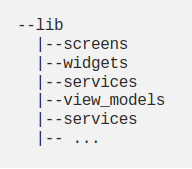
\includegraphics[width=4cm]{../libs/layer-first-tree}
					\caption{Layer first example \cite{scalableFolder}}
					\label{fig: Layer first example}
				\end{figure}
			\end{column}
			\begin{column}{0.6\textwidth}
				\emph{Struttura layer first}
				\newline
				Come intuibile dal nome, questo tipo di struttura si basa su una suddivisione dell'intero progetto in cartelle che contengono i vari componenti di ogni layer;
			\end{column}
		\end{columns}
	\end{minipage}
\end{frame}

%% ---------------------------------------------------------------------------

\begin{frame}{Feature first}
	\begin{minipage}[0.2\textheight]{\textwidth}
		\begin{columns}[T]
			\begin{column}{0.4\textwidth}
				\begin{figure}[htpb]
					\centering
					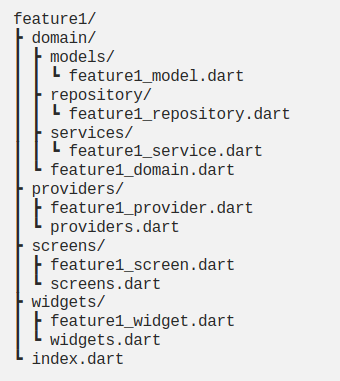
\includegraphics[width=4cm]{../libs/feature-first-tree}
					\caption{Feature first example \cite{scalableFolder}}
					\label{fig: Feature first example}
				\end{figure}
			\end{column}
			\begin{column}{0.6\textwidth}
				\emph{Struttura feature first}
				\newline
				Questo approccio è adatto a progetti grandi, scala molto bene mantenendo una struttura pulita e organizzata.
				Il concetto base è la creazione di una cartella per ogni funzionalità dell'applicativo.
				Come si può notare dall'immagine, ogni cartella conterrà un mini progetto in "Layer First".
			\end{column}
		\end{columns}
	\end{minipage}
\end{frame}

%% ---------------------------------------------------------------------------

\section{Widgets}
\begin{frame}{La base di ogni applicativo in Flutter: il \emph{Widget}}
	\emph{Possiamo individuarne diversi tipi:}
	\begin{itemize}
		\item Widget per l'impostazione di Applicazione o Pagina;
		\item Widget di Layout;
		\item Widget wrapper per contenuti;
		\item Widget per la renderizzazione di liste di elementi;
		\item Widget per l'input da parte dell'utente...
	\end{itemize}
	\emph{Facciamo sempre riferimento al catalogo}
	\newline
	\centering
	\href{https://docs.flutter.dev/development/ui/widgets}{\beamergotobutton{Catologo}}
\end{frame}

%% ---------------------------------------------------------------------------

\begin{frame}{Categorie di widgets}
	\begin{figure}[htpb]
		\centering
		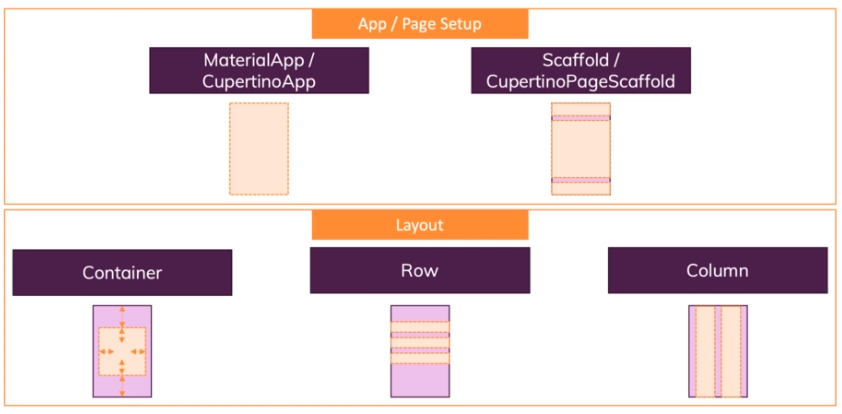
\includegraphics[width=9cm]{../libs/widget-categories-1}
	\end{figure}
\end{frame}

%% ---------------------------------------------------------------------------

\begin{frame}{Categorie di widgets}
	\begin{figure}[htpb]
		\centering
		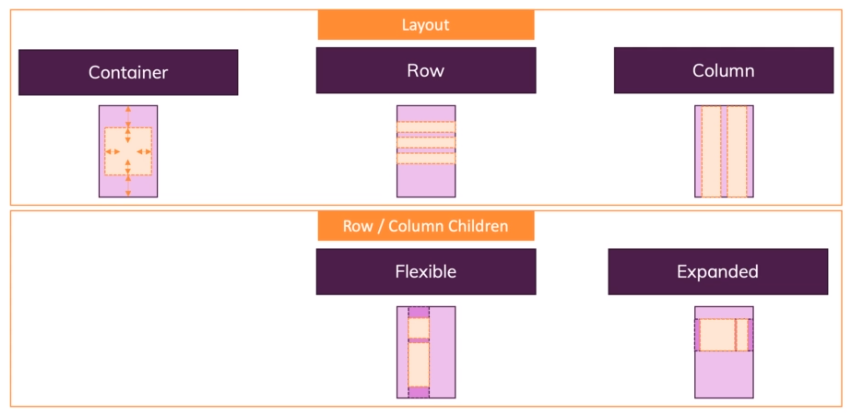
\includegraphics[width=9cm]{../libs/widget-categories-2}
	\end{figure}
\end{frame}

%% ---------------------------------------------------------------------------

\begin{frame}{Categorie di widgets}
	\begin{figure}[htpb]
		\centering
		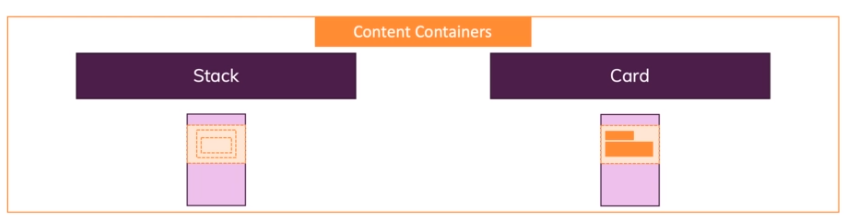
\includegraphics[width=9cm]{../libs/widget-categories-3}
	\end{figure}
\end{frame}

%% ---------------------------------------------------------------------------

\begin{frame}{Categorie di widgets}
	\begin{figure}[htpb]
		\centering
		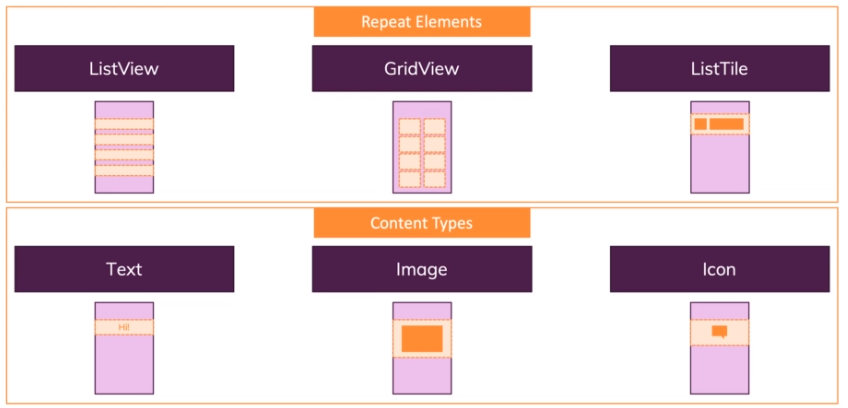
\includegraphics[width=9cm]{../libs/widget-categories-4}
	\end{figure}
\end{frame}

%% ---------------------------------------------------------------------------

\begin{frame}{Categorie di widgets}
	\begin{figure}[htpb]
		\centering
		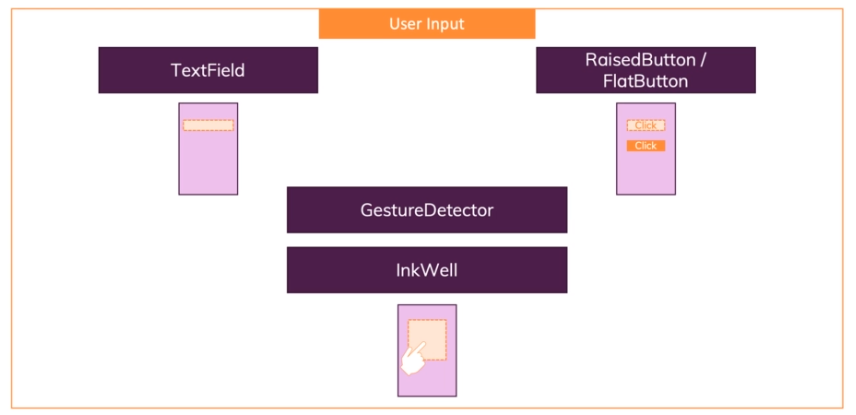
\includegraphics[width=9cm]{../libs/widget-categories-5}
	\end{figure}
\end{frame}

%% ---------------------------------------------------------------------------

\begin{frame}{Widgets colonna e riga}
	\begin{figure}[htpb]
		\centering
		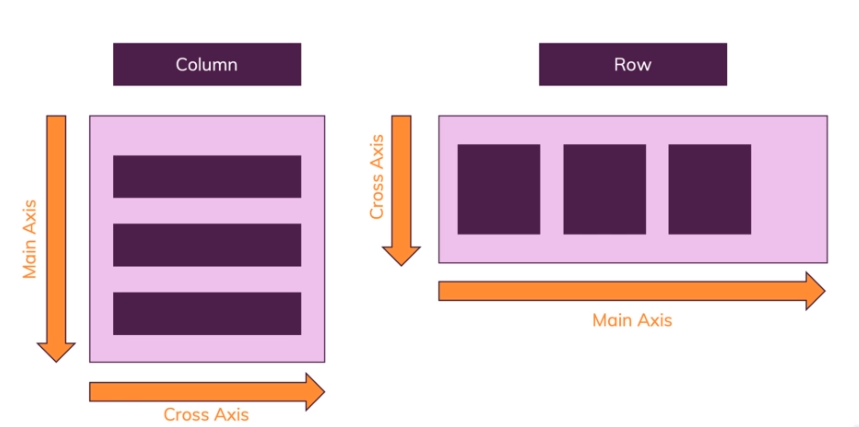
\includegraphics[width=9cm]{../libs/row-column-widgets}
	\end{figure}
\end{frame}

%% ---------------------------------------------------------------------------

\begin{frame}{Combinare i widget}
	\centering
	Non sempre si trova il widget perfetto per il caso d'uso. Analizzali singolarmente e combinali.
	\newline
	\emph{Un esempio:}
	\newline
	\begin{minipage}[0.2\textheight]{\textwidth}
		\begin{columns}[T]
			\begin{column}{0.5\textwidth}
				\emph{Container}
				\begin{itemize}
					\item Riceve esattamente un figlio;
					\item Molte opzioni per lo stile
					\item Perfetto se cerchiamo alta customizzazione
				\end{itemize}
			\end{column}
			\begin{column}{0.5\textwidth}
				\emph{Colonna/Riga}
				\begin{itemize}
					\item Riceve figli multipli;
					\item Nessuna opzione di stile
					\item Prendono sempre tutto lo spazio disponibile nella loro main direction
					\item Perfetto se cerchiamo un allineamento tra più widget
				\end{itemize}
			\end{column}
		\end{columns}
	\end{minipage}
\end{frame}

%% ---------------------------------------------------------------------------

\begin{frame}{Lavorare con le liste}
	\emph{Per renderizzare elementi multipli possiamo considerare due widgets:}
	\begin{itemize}
		\item ListView;
		\item GridView;
	\end{itemize}
\end{frame}

%% ---------------------------------------------------------------------------

\begin{frame}{Renderizzazione liste}
	\emph{ListView e GridView hanno due modalità di utilizzo: }
	\newline
	\begin{figure}[htpb]
		\centering
		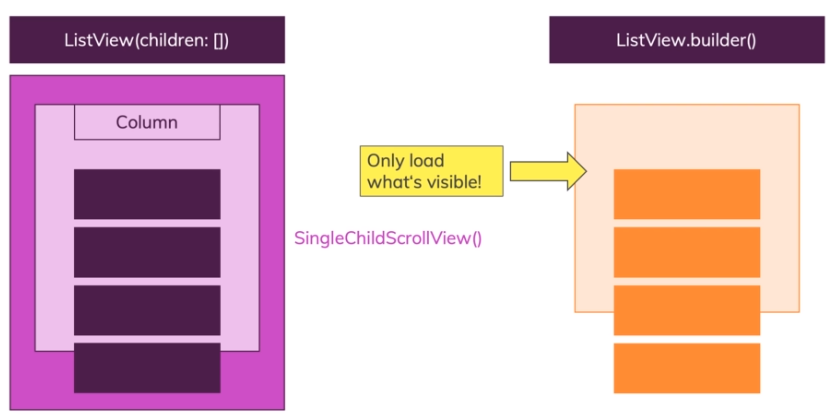
\includegraphics[width=9cm]{../libs/list-view-utilization}
	\end{figure}
\end{frame}


%% ---------------------------------------------------------------------------

\section{Stile}
\begin{frame}{Per le distanze valgono le stesse regole del CSS}
	\begin{figure}[htpb]
		\centering
		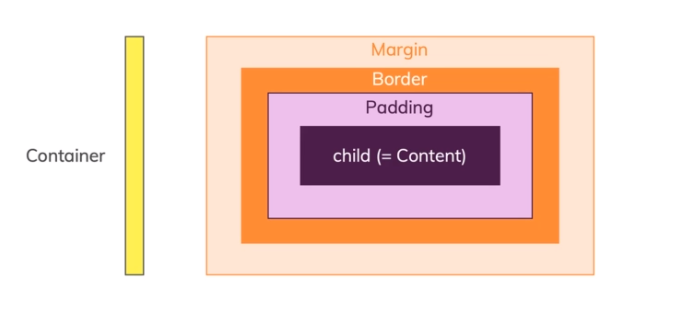
\includegraphics[width=9cm]{../libs/container-style}
	\end{figure}
\end{frame}

%% ---------------------------------------------------------------------------

\begin{frame}{Customizzare lo stile}
	\emph{Possiamo applicare lo stile in due modi:}
	\begin{itemize}
		\item Ogni widget accetta lo stile nel costruttore;
		\item Creare un tema globale per l'applicativo, la maggior parte dei widget faranno riferimento ad esso per gli elementi contenuti;
	\end{itemize}
	\emph{Come sempre, fare riferimento al catalogo}
	\newline
	\centering
	\href{https://docs.flutter.dev/development/ui/widgets}{\beamergotobutton{Catologo}}
\end{frame}

%% ---------------------------------------------------------------------------

\begin{frame}{Tema globale}
	\emph{Utilizzare un tema globale:}
	\begin{itemize}
		\item Come linea guida di uno stile uniforme in tutta l'applicazione;
		\item I widget seguono per le proprie caratteristiche lo stile configurato nel tema;
	\end{itemize}
	\centering
	\href{https://api.flutter.dev/flutter/material/ThemeData-class.html}{\beamergotobutton{Documentazione}}
\end{frame}

%% ---------------------------------------------------------------------------

\section{Esercitazione}
\begin{frame}{Migliorare la precedente esercitazione}
\begin{minipage}[0.2\textheight]{\textwidth}
		\begin{columns}[T]
			\begin{column}{0.4\textwidth}
				\begin{figure}[htpb]
					\centering
					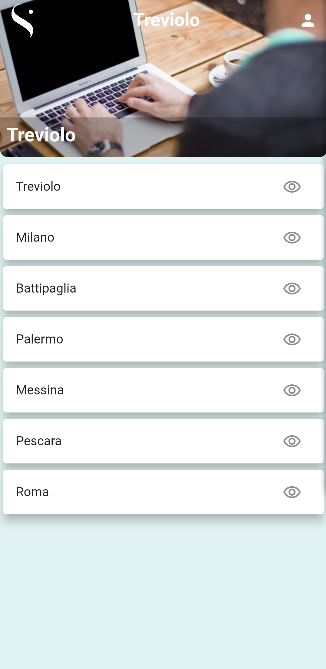
\includegraphics[width=2cm]{../libs/assignment-2-home}
				\end{figure}
			\end{column}
			\begin{column}{0.6\textwidth}
				\emph{Alcuni spunti:}
				\begin{itemize}
					\item Creare un tema globale per l'app;
					\item Utilizzare ListView e ListTile;
					\item Inserire il logo di SI nel logo;
					\item Creare un'area in cima che visualizzi la sede selezionata, inserire bordi arrotondati nella parte inferiore;
					\item ogni elemento avrà un'immagine presa dal web, inserirla come sfondo nella parte superiore;
				\end{itemize}
			\end{column}
		\end{columns}
	\end{minipage}
\end{frame}


%% ---------------------------------------------------------------------------

% Reference frames
\begin{frame}[allowframebreaks]
    \frametitle{Riferimenti}
    \printbibliography
\end{frame}

%% ---------------------------------------------------------------------------
% Final frame
\section{Fine}
\begin{frame}{}
	\huge\emph{Grazie per l'attenzione!}
	\newline
	\vfill
	\hfill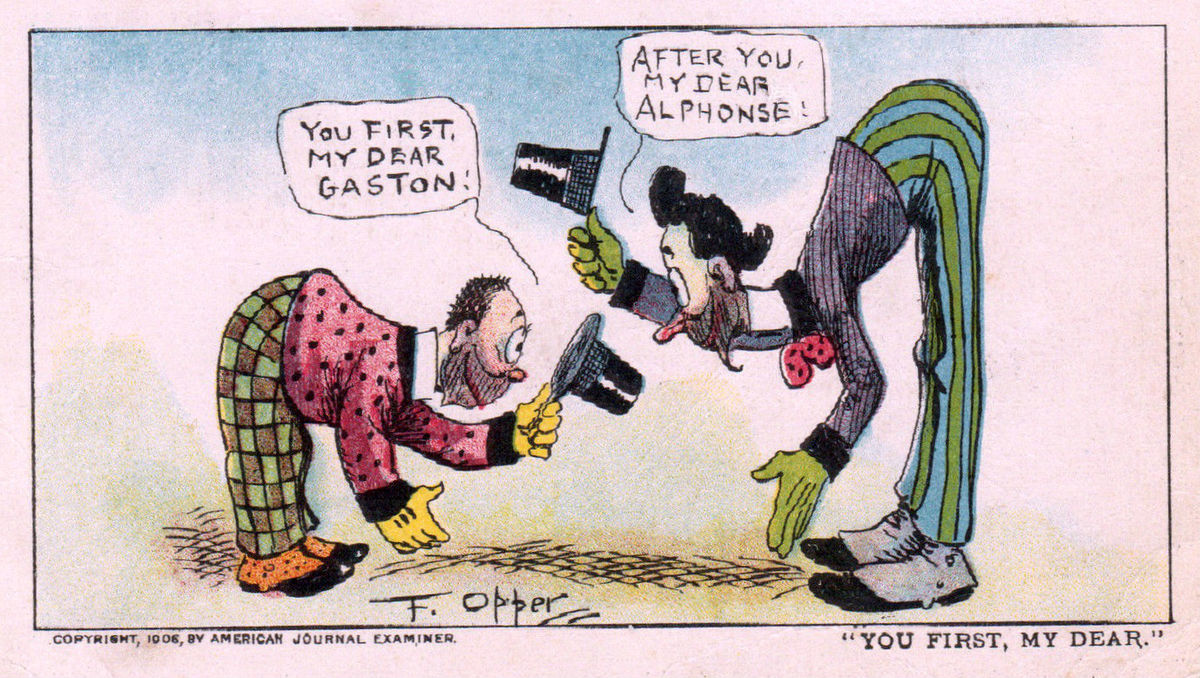
\includegraphics[width=6cm]{../libs/alphonse-gaston-regards}
\end{frame}

\end{document}